\documentclass[12pt]{article}
\usepackage[left=1cm, right=1cm, top=2cm,bottom=1.5cm]{geometry} 

\usepackage[parfill]{parskip}
\usepackage[utf8]{inputenc}
\usepackage[T2A]{fontenc}
\usepackage[russian]{babel}
\usepackage{enumitem}
\usepackage[normalem]{ulem}
\usepackage{amsfonts, amsmath, amsthm, amssymb, mathtools}
\usepackage{tabularx}
\usepackage{hhline}

\usepackage{accents}
\usepackage{fancyhdr}
\pagestyle{fancy}
\renewcommand{\headrulewidth}{1.5pt}
\renewcommand{\footrulewidth}{1pt}

\usepackage{graphicx}
\usepackage[figurename=Рис.]{caption}
\usepackage{subcaption}
\usepackage{float}

%%Наименование папки откуда забирать изображения
\graphicspath{ {./images/} }

%%Изменение формата для ввода доказательства
\renewcommand{\proofname}{$\square$  \nopunct}
\renewcommand\qedsymbol{$\blacksquare$}

%%Изменение отступа на таблицах
\addto\captionsrussian{%
	\renewcommand{\proofname}{$\square$ \nopunct}%
}
%% Римские цифры
\newcommand{\RN}[1]{%
	\textup{\uppercase\expandafter{\romannumeral#1}}%
}

%% Для удобства записи
\newcommand{\MR}{\mathbb{R}}
\newcommand{\MC}{\mathbb{C}}
\newcommand{\MQ}{\mathbb{Q}}
\newcommand{\MN}{\mathbb{N}}
\newcommand{\MTB}{\mathbb{T}}
\newcommand{\MTI}{\mathbb{I}}
\newcommand{\MI}{\mathrm{I}}
\newcommand{\MJ}{\mathrm{J}}
\newcommand{\MH}{\mathrm{H}}
\newcommand{\MT}{\mathrm{T}}
\newcommand{\MU}{\mathcal{U}}
\newcommand{\MV}{\mathcal{V}}
\newcommand{\MB}{\mathcal{B}}
\newcommand{\MW}{\mathcal{W}}
\newcommand{\ML}{\mathcal{L}}
\newcommand{\VN}{\varnothing}
\newcommand{\VE}{\varepsilon}

\theoremstyle{definition}
\newtheorem{defn}{Опр:}
\newtheorem{rem}{Rm:}
\newtheorem{prop}{Утв.}
\newtheorem{exrc}{Упр.}
\newtheorem{lemma}{Лемма}
\newtheorem{theorem}{Теорема}
\newtheorem{corollary}{Следствие}

\newenvironment{cusdefn}[1]
{\renewcommand\thedefn{#1}\defn}
{\enddefn}

\DeclareRobustCommand{\divby}{%
	\mathrel{\text{\vbox{\baselineskip.65ex\lineskiplimit0pt\hbox{.}\hbox{.}\hbox{.}}}}%
}
%Короткий минус
\DeclareMathSymbol{\SMN}{\mathbin}{AMSa}{"39}
%Длинная шапка
\newcommand{\overbar}[1]{\mkern 1.5mu\overline{\mkern-1.5mu#1\mkern-1.5mu}\mkern 1.5mu}
%Функция знака
\DeclareMathOperator{\sgn}{sgn}

%Функция ранга
\DeclareMathOperator{\rk}{\text{rk}}

%Обозначение константы
\DeclareMathOperator{\const}{\text{const}}

\DeclareMathOperator*{\dsum}{\displaystyle\sum}
\newcommand{\ddsum}[2]{\displaystyle\sum\limits_{#1}^{#2}}

%Интеграл в большом формате
\DeclareMathOperator{\dint}{\displaystyle\int}
\newcommand{\ddint}[2]{\displaystyle\int\limits_{#1}^{#2}}
\newcommand{\ssum}[1]{\displaystyle \sum\limits_{n=1}^{\infty}{#1}_n}

\newcommand{\smallerrel}[1]{\mathrel{\mathpalette\smallerrelaux{#1}}}
\newcommand{\smallerrelaux}[2]{\raisebox{.1ex}{\scalebox{.75}{$#1#2$}}}

\newcommand{\smallin}{\smallerrel{\in}}
\newcommand{\smallnotin}{\smallerrel{\notin}}

\newcommand*{\medcap}{\mathbin{\scalebox{1.25}{\ensuremath{\cap}}}}%
\newcommand*{\medcup}{\mathbin{\scalebox{1.25}{\ensuremath{\cup}}}}%

\makeatletter
\newcommand{\vast}{\bBigg@{3.5}}
\newcommand{\Vast}{\bBigg@{5}}
\makeatother

%Промежуточное значение для sup\inf, поскольку они имеют разную высоту
\newcommand{\newsup}{\mathop{\smash{\mathrm{sup}}}}
\newcommand{\newinf}{\mathop{\mathrm{inf}\vphantom{\mathrm{sup}}}}

%Скалярное произведение
\DeclarePairedDelimiterX{\inner}[2]{\langle}{\rangle}{#1, #2}

%Подпись символов снизу
\newcommand{\ubar}[1]{\underaccent{\bar}{#1}}

%% Шапка для букв сверху
\newcommand{\wte}[1]{\widetilde{#1}}

%%Функция для обозначения равномерной сходимости по множеству
\newcommand{\uconv}[1]{\overset{#1}{\rightrightarrows}}
\newcommand{\uconvm}[2]{\overset{#1}{\underset{#2}{\rightrightarrows}}}

%%Функция для обозначения нижнего и верхнего интегралов
\def\upint{\mathchoice%
	{\mkern13mu\overline{\vphantom{\intop}\mkern7mu}\mkern-20mu}%
	{\mkern7mu\overline{\vphantom{\intop}\mkern7mu}\mkern-14mu}%
	{\mkern7mu\overline{\vphantom{\intop}\mkern7mu}\mkern-14mu}%
	{\mkern7mu\overline{\vphantom{\intop}\mkern7mu}\mkern-14mu}%
	\int}
\def\lowint{\mkern3mu\underline{\vphantom{\intop}\mkern7mu}\mkern-10mu\int}


\begin{document}
\lhead{Математический анализ - \RN{3}}
\chead{Шапошников С.В.}
\rhead{Лекция - 18}
\section*{Производящие функции}
Производящие функции очень часто используются в комбинаторике, теории вероятностей, физике и алгоритмах программирования. 

\begin{defn}
	Пусть у нас есть последовательность $\{a_n\}_{n = 0}^{\infty}$, тогда ей можно сопоставить следующую формальную сумму (в том смысле, что мы не предполагаем, что это сумма сходится):
	$$
		A(z) = \ddsum{n = 0}{\infty}a_n z^n
	$$
	Этот объект называется \uwave{производящей функцией}.
\end{defn}

С такими суммами можно выполнять формальные операции (то есть как-будто мы делаем некоторую операцию с последовательностью). Можно думать об этом так: вместо последовательности мы зачем-то начали писать суммы, определенные выше.  

Пусть $A(z) = \ddsum{n = 0}{\infty}a_n z^n, \, B(z) = \ddsum{n = 0}{\infty}b_n z^n$, тогда определим формальные операции над ними:

\textbf{1) \uline{Сложение}}: $\alpha A(z) + \beta B(z) = \ddsum{n = 0}{\infty}\left(\alpha a_n + \beta b_n\right)z^n$;

\textbf{2) \uline{Умножение}}: $A(z){\cdot}B(z) = \ddsum{n = 0}{\infty}\left(a_0 b_n + a_1 b_{n-1} + \dotsc + a_n b_0\right)z^n$;

\textbf{3) \uline{Дифференцирование}}: $A^\prime(z) = \ddsum{n = 1}{\infty}n a_n z^{n-1}$;

\textbf{4) \uline{Интегрирование}}: $\displaystyle \int  A(z)dz = \ddsum{n = 1}{\infty}\dfrac{a_n}{n+1}z^{n+1} + \const$;

Каждое из этих действий оставляет нас в рамках действий с последовательностями. Раньше, последовательности можно было складывать, а теперь, благодоря степенным рядам, возникает набор нетривиальных действий с ними: перемножение, дифференцирование, интегрирование. Эти действия естественны с точки зрения степенных рядов. Если где-то такие степенные ряды сошлись, то на общем круге сходимости эти операции - честные операции, то есть совсем обычные операции, а не формальные. 

На круге сходимости определена функция $A(z)$ и она содержит всю информацию про последовательность $\{a_n\}$: если радиус сходимости $R > 0$, то мы можем вычислять её члены следующим образом:
$$
	\forall n \in \MN, \, a_n = \dfrac{A^{(n)}(0)}{n!}
$$
Следовательно функция $A(z)$ составлена по последовательности и зная её можно эту последовательность найти. В этом смысле, $A(z)$ как бы ``производит'' последовательность, порождает её как последовательность своих коэффициентов Тейлора в нуле. Далее, рассмотрим примеры таких функций.

\newpage
\section*{Применение производящих функций}
\subsection*{$(\RN{1})$ Числа Фибоначчи}
Числа Фибоначчи определяются следующим образом: $f_0 = f_1 = 1, f_{n+1} = f_n + f_{n-1}$. Попробуем найти производящую функцию $F(z)$ этой последовательности:
$$
	F(z) = \ddsum{n = 0}{\infty}f_n z^n = 1 + z + \ddsum{n = 2}{\infty}(f_{n-1} + f_{n-2})z^n = 1 + z + z\left(\ddsum{n = 2}{\infty}f_{n -1}z^{n-1}\right) + z^2\left(\ddsum{n = 2}{\infty}f_{n-2}z^{n-2}\right) =
$$
$$
	= 1 + z + z(F(z) - 1) + z^2F(z) = 1 + z F(z) + z^2 F(z) \Rightarrow 
$$
$$	
	\Rightarrow (1 - z - z^2)F(z) = 1 \Rightarrow F(z) = \dfrac{1}{1 - z - z^2}
$$
Теперь можно разложить производящую функцию в степенной ряд используя её явный вид:
$$
	z^2 + z - 1 = 0 \Rightarrow z_1,z_2 = \dfrac{-1 \pm \sqrt{5}}{2} \Rightarrow F(z) = \dfrac{-1}{(z_1 - z)(z_2 - z)} = \dfrac{-1}{z_2 - z_1}\left(\dfrac{1}{z_1 - z} - \dfrac{1}{z_2 - z}\right)
$$
Вынесем $z_1$ и $z_2$ за скобки и используем сумму бесконечной геометрической прогрессии, тогда:
$$
	F(z) = \dfrac{-1}{z_2 - z_1}\left(\dfrac{1}{z_1}{\cdot}\dfrac{1}{1 - \frac{z}{z_1}} - \dfrac{1}{z_2}{\cdot}\dfrac{1}{1 - \frac{z}{z_2}}\right) = \dfrac{-1}{z_2 - z_1}\left(\dfrac{1}{z_1}{\cdot}\ddsum{n = 0}{\infty}\dfrac{z^n}{z_1^n} - \dfrac{1}{z_2}{\cdot}\ddsum{n = 0}{\infty}\dfrac{z^n}{z_2^n}\right) =
$$
$$
	=	\ddsum{n = 0}{\infty}\left(\dfrac{1}{z_2 - z_1}{\cdot}\left(\dfrac{1}{z_2^{n+1}} - \dfrac{1}{z_1^{n+1}}\right)\right)z^n
$$
Мы получили так называемую \uwave{формулу Бине}.

Число Фибоначчи удовлетворяло простому реккурентному соотношению (такие соотношения называются \uwave{линейными}): $f_{n+1} = f_n + f_{n-1}$. 
\begin{enumerate}[label=(\arabic*)]
	\item Если найти две последовательности, которые удовлетворяют такому соотношению, то их сумма тоже будет удовлетворять такому соотношению;
	
	\item  Если найти последовательность удовлетворяющую такому соотношению и умножить её на число, то опять получится последовательность удовлетворяющая этому соотношению;
\end{enumerate}
Мы посчитали производяющую функцию и она оказалась рациональной дробью. Оказывается, что это общий факт: всегда при работе с линейными реккурентными соотношениями в качестве производящей функции мы будем получать рациональные дроби.

\begin{prop}\hfill
	\begin{enumerate}[label=\arabic*)]
		\item 	Пусть $\{a_n\} \colon a_{n+1} = c_1 a_n + c_2 a_{n-1} + \dotsc + c_k a_{n -k + 1}$, тогда производящая функция это дробь:
		$$
			A(z) = \dfrac{P(z)}{Q(z)}, \, \deg{Q} = k, \, \deg{P} \leq k-1
		$$
		\item Если производящая функция это дробь: 
		$$
			A(z) = \dfrac{P(z)}{Q(z)}, \, Q(z) = 1 + c_1 z + \dotsc
		$$ 
		то начиная с некоторого номера $a_n$ удовлетворяет линейному реккурентному соотношению;
	\end{enumerate}
\end{prop}
\begin{proof}\hfill
	\begin{enumerate}[label=\arabic*)]
		\item Умножим $A(z)$ на разложенное $c_1 z + c_2 z^2 + \dotsc + c_kz^k$ и соберем коэффициент при $z^n, \, n \geq k$:
		$$
			z^n, \, n \geq k \colon c_1 a_{n-1} + c_2 a_{n-2} + \dotsc + c_k a_{n - k} = a_n \Rightarrow 
		$$
		$$
			\Rightarrow (c_1 z + c_2 z^2 + \dotsc + c_kz^k)A(z) = A(z) + P(z), \, \deg{P} \leq k -1 \Rightarrow
		$$
		$$
			\Rightarrow A(z) = \dfrac{P(z)}{c_1 z + c_2 z^2 + \dotsc + c_kz^k - 1} = \dfrac{P(z)}{Q(z)}, \, \deg{Q} = k
		$$
		\item Домножим $A(z)$ на $Q(z)$ и приравняем коэффициенты:
		$$
			Q(z){\cdot}A(z) = (1 + c_1 z + \dotsc ){\cdot}A(z) = P(z) \Rightarrow P(z) - A(z) = A(z)(c_1 z + \dotsc )
		$$
		Пусть степень многочлена $P(z)$ равна $m$ и $P(z) = \ddsum{n = 0}{\infty}b_n z^n \Rightarrow \forall n > m, \, b_n = 0$, тогда:
		$$
			\forall n \geq m + 1, \, z^n \colon - a_n = c_1 a_{n-1} + c_2 a_{n - 2} + \dotsc + c_{m  + 1}a_{n - (m +1)}
		$$
	\end{enumerate}
\end{proof}

\textbf{Пример}: в кармане есть только один рубль и пять рублей, сколькими способами можно разменять $n$ рублей? На самом деле можно выбрать любое число монет. Рассмотрим следующее выражение:
$$
	(1 + z + z^2 + z^3 + \dotsc)(1 + z^5 + z^{10} + z^{15} + \dotsc ) = \ddsum{n = 0}{\infty}a_n z^n
$$
где равенство получается раскрытием скобок и сбором слагаемых по степеням. При степени $z^n$ будет стоять $a_n$ - число слагаемых, полученное взятием какого-то числа слагаемых из левой скобки и какого-то числа слагаемых из правой скобки. Число $a_n$ это в точности число способов разменять $n$ по рублю и по пять рублей. Попробуем найти эти $a_n$:
$$
	(1 + z + z^2 + z^3 + \dotsc)(1 + z^5 + z^{10} + z^{15} + \dotsc ) = \dfrac{1}{(1 - z)(1-z^5)} = \dfrac{1}{1 - z - z^5 + z^6} = A(z) \Rightarrow
$$
$$
	\Rightarrow (1 - z - z^5 + z^6)A(z) = 1 \Rightarrow \forall n \geq 6, \, z^n: a_n - a_{n-1} - a_{n -5} + a_{n -6} = 0 
$$
Таким образом, мы получаем ответ: $a_n = a_{n-1} + a_{n -5} - a_{n -6}$.

\begin{exrc}
	Посчитать с помощью производящих функций следующую сумму: $(C_n^0)^2 + \dotsc + (C_n^n)^2$.
\end{exrc}
\begin{proof}
	Рассмотрим Бином Ньютона и его производящую функцию:
	$$
		(1 + z)^n = \ddsum{k = 0}{n}C_n^k z^k = \ddsum{k = 0}{\infty}a_k z^k = A(z), \,  a_k = C_n^k, \forall k = \overline{0,n}, \, a_k = 0, \forall k > n
	$$
	Рассмотрим следующее произведение двух биномов Ньютона:
	$$
		(1 + z)^n(z + 1)^n = (C_n^0 + C_n^1 z + C_n^2 z^2 + \dotsc + C_n^n z^n){\cdot}(C_n^0z^n + C_n^1 z^{n-1} + C_n^2 z^{n-2}  + \dotsc + C_n^n ) = A^2(z)
	$$
	где мы можем раскрыть скобки и собрать слагаемые, затем рассмотрим $B(z) = (A(z))^2$:
	$$
		B(z) = (A(z))^2 = (1 + z)^{2n} = \ddsum{k = 0}{2n}C_{2n}^k z^k = \ddsum{k = 0}{\infty}a_k z^k \Rightarrow a_n = C_{2n}^n = (C_n^0)^2 + (C_n^1)^2 + \dotsc + (C_n^n)^2
	$$
\end{proof}
\newpage
\subsection*{$(\RN{2})$ Числа Каталана}
Когда пишется алгебраическое выражение, оно содержит скобки, которые указывают последовательность действий. Из таких выражений можно удалить всё кроме скобок, то что получится будет называться \uwave{скобочной структурой}. Например:
$$
	((1{\cdot}2) + (3{\cdot}(1 + 2))) \mapsto (() \, (\, ()))
$$
Скобочные структуры бывают правильные и неправильные. Правильная  скобочная структура в начале имеет число левых скобок $\geq$ число правых скобок, а по всему выражению число левых скобок $=$ числу правых скобок. 

Пусть у нас всего $n$ пар скобок, сколько правильных скобочных структур $c_n$ можно построить?
$$
	c_1 \colon () \Rightarrow c_1 = 1, \, c_2 \colon ()(), (()) \Rightarrow c_2 = 2
$$
Возьмем скобочную структуру из $n+1$ пары скобок. Будем считать $c_0 = 1$. Возьмем $1$-ую левую скобку и посмотрим, где она закрывается: может оказаться так, что справа от закрывающей скобки ничего нет, может оказаться, что внутри $k$ пар скобок, а за правой скобокой находится $(n-k)$ структур:
$$
	(\; \underbrace{\hspace{1cm}\dotsc \hspace{1cm}}_k  \;)\; \underbrace{\hspace{1cm}\dotsc \hspace{1cm}}_{n-k} \;
$$
Для каждого фиксированного $k$ может возникнуть $c_k{\cdot}c_{n-k}$ разных скобочных структур. Просуммируем и получим число скобочных структур из $n+1$ пары скобок:
$$
	c_{n+1} = \ddsum{k = 0}{n}c_k{\cdot}c_{n-k} \Rightarrow C(z) = \ddsum{n = 0}{\infty}c_n z^n ?
$$
Теперь интересно найти производящую функцию, вдруг она окажется такой, что  мы умеем по-другому раскладывать её в ряд и тогда сможем узнать, какова формула для $c_n$ или узнаем более простую реккурентную формулу. Возведем $C(z)$ в квадрат:
$$
	C(z)^2 = \ddsum{n = 0}{\infty}\left(c_0 c_n + \dotsc c_n c_0\right)z^n = \ddsum{n = 0}{\infty}c_{n+1}z^n = \dfrac{1}{z} \ddsum{n = 0}{\infty}c_{n+1}z^{n+1} = \dfrac{C(z) - 1}{z} \Rightarrow
$$
$$
	\Rightarrow zC(z)^2 - C(z) + 1 = 0 \Rightarrow C(z) = \dfrac{1 \pm \sqrt{1 - 4z}}{2z}
$$
Ищем $C(z)$ в виде степенного ряда. Поскольку ряд $C(z)$ в нуле равен $0$, то если мы возьмем в решении выше знак $+$, то в нуле мы получим выражение вида $\tfrac{1}{z}$, следовательно для получения степенного ряда нам необходимо, чтобы единцы в числителе сократились $\Rightarrow$ берем знак $-$. Тогда:
$$
	C(z) = \dfrac{1 - \sqrt{1 - 4z}}{2z} = \dfrac{1}{2z}\left(1 - (1 - 4z)^{\tfrac{1}{2}}\right)
$$
Вспомним бином Ньютона при $\alpha = \tfrac{1}{2}, \, t = -4z$:
$$
	(1 + t)^\alpha = \ddsum{n = 0}{\infty}\dfrac{\alpha{\cdot}(\alpha - 1){\cdot}\dotsc{\cdot}(\alpha - n +1)}{n!}{\cdot}t^n = \ddsum{n = 0}{\infty}\dfrac{\tfrac{1}{2}{\cdot}\left(\tfrac{1}{2}-1\right){\cdot}\dotsc{\cdot}\left(\tfrac{1}{2} - n + 1\right)}{n!}{\cdot}(-4)^nz^n \Rightarrow
$$
$$
	\Rightarrow C(z) = \dfrac{1}{2z}\left(1 - (1 - 4z)^{\tfrac{1}{2}}\right) = \ddsum{n = 1}{\infty}\dfrac{\tfrac{1}{4}{\cdot}\left(\tfrac{1}{2}-1\right){\cdot}\dotsc{\cdot}\left(\tfrac{1}{2} - n + 1\right){\cdot}4^n}{n!}(-1)^{n+1}{\cdot}z^{n-1} =
$$
$$
	= \ddsum{n = 1}{\infty}\dfrac{\tfrac{1}{4}{\cdot}\left(1 - \tfrac{1}{2}\right){\cdot}\dotsc{\cdot}\left((n-1) - \tfrac{1}{2} \right){\cdot}(-1)^{n-1}{\cdot}4^n}{n!}(-1)^{n+1}{\cdot}z^{n-1} = \ddsum{n = 1}{\infty}\dfrac{4^{n-1}{\cdot}(1{\cdot}3{\cdot}\dotsc{\cdot}(2n -3))}{2^{n-1}{\cdot}n!}z^{n-1} =
$$
$$
	= \ddsum{n = 1}{\infty}\dfrac{2^{n-1}{\cdot}(n-1)!{\cdot}(1{\cdot}3{\cdot}\dotsc{\cdot}(2n -3))}{n!(n-1)!}z^{n-1} = \ddsum{n = 1}{\infty}\dfrac{(2n-2)!}{n!(n-1)!}z^{n-1} = \ddsum{n = 1}{\infty}\dfrac{1}{n}C_{2n -2}^{n-1}z^{n-1} \Rightarrow
$$
$$
	\Rightarrow c_{n-1} = \dfrac{1}{n}C_{2n -2}^{n-1}z^{n-1} \Rightarrow c_n = \dfrac{1}{n+1}C_{2n}^n
$$
\begin{rem}
	Что-то очень похожее могло возникать при анализе теоремы Муавра-Лапласа ранее.
\end{rem}

\subsection*{Число триангуляций}

Числа Каталана, помимо исходной задачи, дают ответ на другие. С помощью них можно решить задачу про число триангуляций: возьмем выпуклый $(n+2)$-угольник и начинаем диагоналями разбивать на треугольники, чтобы диагонали пересекались только в вершинах. Сколько таких разбиений может быть? У $(n+2)$-угольника таких может быть $c_n$. Будем считать, что $c_0 = 1$. 
\begin{figure}[H]
	\centering
	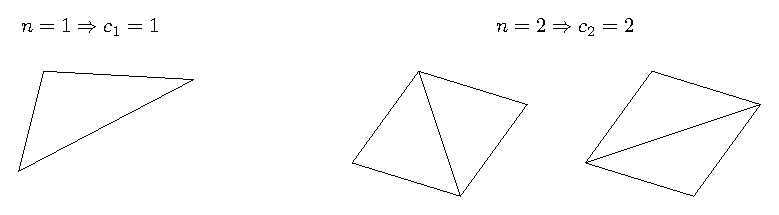
\includegraphics[width=0.75\textwidth]{MA3L18_1.eps}
	\label{MA3L18_1}
	\caption{Число триангуляция для случаев $n = 1$ и $n = 2$.}
	\label{fig:число триангуляций}
\end{figure}
Можно попробовать опять получить реккурентную формулу и убедиться, что она получится такой же, как и для скобочных структур: выделим какую-то фиксированную сторону $\Rightarrow$ триангуляцией выделяется треугольник, который эту сторону содержит. 
\begin{figure}[H]
	\centering
	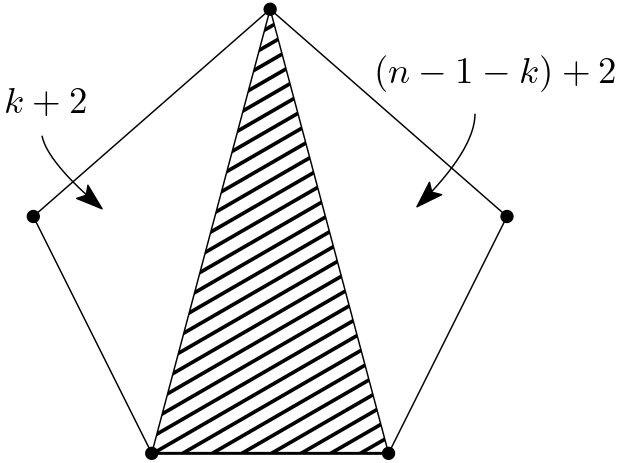
\includegraphics[width=0.35\textwidth]{MA3L18_2.png}
	\label{MA3L18_2}
	\caption{Число триангуляций при фиксированной стороне.}
	\label{fig: триангуляции}
\end{figure}
Тогда можно заметить, что если слева от построенного треугольника образовался $(k+2)$-угольник, то справа образовался $((n - 1 - k) + 2)$-угольник, следовательно слева мы получили $c_k$ способов триангуляции, а справа $c_{(n - 1) - k}$. Перебираем все способы, тогда мы опять получим знакомое реккурентное соотношение:
$$
	c_n = \ddsum{k = 0}{n - 1}c_k{\cdot}c_{(n - 1) - k } \Rightarrow c_n = \dfrac{1}{n+1}C_{2n}^n
$$

\subsection*{Пути Дика}
Аналогичной задачей, является поиск числа путей от точки $0$ до $2n$, если разрешено проводить ломанные под углом в $45^\circ$ вверх и вниз, не выходя ниже оси абсцисс.  
\begin{figure}[H]
	\centering
	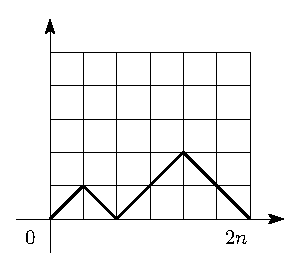
\includegraphics[width=0.35\textwidth]{MA3L18_3.eps}
	\label{MA3L18_3}
	\caption{Число путей Дика.}
	\label{fig:пути Дика}
\end{figure}
Данная задача однозначно сопоставляется с задачей про скобки. Когда идем наверх скобка открывается, когда идем вниз скобка закрывается. Поэтому каждая скобочная структура может быть определена такой ломаной. Следовательно и путей всего может быть $c_{n}$.

\begin{rem}
	Книга Ландо ``Производящие функции'' содержит большое количество примеров, связанных с производящими функциями.
\end{rem}

\subsection*{$(\RN{3})$ Многочлены Лежандра}
Есть материальная точка $x_0$ с массой $m_0$ и есть другая материальная точка $x$ с массой $m$. Спрашивается с какой силой точка $(x,m)$ притягивается к $(x_0,m_0)$. Вспоминая формулу из физики:
$$
	F = - \dfrac{\gamma m m_0 (x - x_0)}{|x - x_0|^3}
$$
У силы есть потенциал (то из чего дифференцированием, получилась сила) $U$:
$$
	U = \dfrac{\gamma m m_0}{|x - x_0|}, \, F = \nabla U
$$
Что будет, если у точек очень много $(x_j, m_j)$ и все притягивают точку $(x,m)$. Рассмотрим:
$$
	U = \ddsum{j}{}\dfrac{\gamma m m_j}{|x - x_j|}
$$
Если эти точки находятся достаточно удаленно, то может быть не видно, что там множество точек и физиками было предложено взять центр масс, в который собирается вся масса и считать, что это одна точка, которая притягивает. Это означает, что мы хотим заменить потенциал примерно следующим выражением:
$$
	U = \ddsum{j}{}\dfrac{\gamma m m_j}{|x - x_j|} \sim \dfrac{\gamma m {\cdot}\sum\limits_{j}m_j}{|x - x_0|}
$$
Возникает естественный вопрос, а какова погрешность таких замен? Что происходит, когда мы так заменяем? Собственно этим вопросом когда-то задался Лежандр. Возьмем какой-либо $y$ среди этих точек и попробуем осознать, какое же получится отличие. Пусть расстояние между $y$ и $x_0$ равно $r_0$, расстояние между $x$ и $x_0$ равно $r$, а угол между $x x_0$ и $y x_0$ равен $\theta$.

\begin{figure}[H]
	\centering
	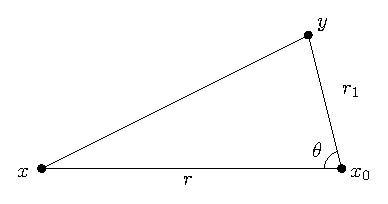
\includegraphics[width=0.55\textwidth]{MA3L18_4.eps}
	\label{MA3L18_4}
	\caption{Оценка замены точек $x_j$ центром масс $x_0$.}
	\label{fig:замена точек центром масс}
\end{figure}
Пусть $t = \cos{\theta}$, тогда по теореме косинусов $|x -y| = \sqrt{r^2 + r_1^2 - 2r_1 r t}$, также обозначим $\alpha = \tfrac{r_1}{r}$. Поскольку считаем, что до массы точек расстояние очень большое (летает далеко), то $\alpha <1$. Тогда:
$$
	|x - y| = \sqrt{r^2 + r_1^2 - 2r_1 r t} = r\sqrt{ 1 + \alpha^2 - 2\alpha t} \Rightarrow \dfrac{1}{|x - y|} = \dfrac{1}{r}{\cdot}\dfrac{1}{\sqrt{1 + \alpha^2 - 2\alpha t}} = \dfrac{1}{r}{\cdot}(*)
$$
Поскольку $\alpha$ - мало, разложим последнее выражение в степенной ряд, обозначив коэффициенты $P_n(t)$:
$$
	\dfrac{1}{|x - y|} = \dfrac{1}{r}{\cdot}\dfrac{1}{\sqrt{1 + \alpha^2 - 2\alpha t}} = \dfrac{1}{r}\ddsum{n = 0}{\infty}P_n(t)\alpha^n , \, P_0(t) = 1
$$
Подставим это выражение в формулу потенциала для каждой точки и распишем асимптотику:
$$
	U = \ddsum{j}{}\dfrac{\gamma m m_j}{r}\ddsum{n = 0}{\infty}\dfrac{r_j^n}{r^n}P_n(t_j) = \dfrac{\gamma m \sum\limits_{j}m_j}{r} + \dfrac{\gamma m }{r^2}\ddsum{j}{}m_j r_j P_1(t_j) + \dotsc
$$
Коэффициенты $P_n(t)$ это многочлены по $t$, обладающие многими хорошими свойствами, они называются \uwave{многочленами Лежандра}. Видно, что эти многочлены Лежандра появляются также как появлялись последовательности: с помощью производящей функции $(*) \Rightarrow$ можно порождать функциональные последовательни. Попробуем понять, как устроены эти многочлены. Продифференцируем $(*)$:
$$
	\left(\dfrac{1}{\sqrt{1 + \alpha^2 - 2\alpha t}}\right)^\prime = \dfrac{-\alpha + t}{(1 + \alpha^2 - 2\alpha t)\sqrt{1 + \alpha^2 - 2\alpha t}} = \ddsum{n = 1}{\infty}nP_n(t)\alpha^{n-1 } \Rightarrow
$$
$$
	\Rightarrow (t-\alpha)\ddsum{n = 0}{\infty}P_n(t)\alpha^n = (1 + \alpha^2 - 2\alpha t)\ddsum{n = 1}{\infty}nP_n(t)\alpha^{n-1 }
$$
И приравниваем коэффициенты при слагаемых с обеих сторон:
$$
	\alpha_n \colon tP_n(t) - P_{n-1}(t) = (n + 1)P_{n+1}(t) + (n-1)P_{n-1}(t) - 2n tP_n(t)
$$
Приведем подобные и получим:
$$
	(n+1)P_{n+1}(t) = (1 + 2n)tP_n(t) - nP_{n-1}(t)
$$
Видно, что если первые два коэффициента это многочлены, то дальше будут только многочлены.
\end{document}